\chapter{Empirical Evaluation}
\label{chap:evaluation}

We test several hypotheses in order to provide a thorough comparison of CPU versus GPU processing as well as online versus offline learning. This chapter contains detailed explanations of each experiment we ran, including why we ran the experiment, the environment setup, and a discussion of the results.

\section{Agent Reward}

To evaluate the viability of our Quake III bot implementation we measured the cumulative reward of each test scenario. A summary of the data we collected is available in Table \ref{tab:reward}. The table tracks the average reward per action for the LSPI agent under different configurations. All of the tests were completed by evaluating our agent against a native bot in a deathmatch to $50$. Every test used the same map, difficulty setting, and bots. The same discount factor of $0.95$ was used for all tests.

\begin{table}%
    \centering
    \begin{tabular}{|c|c|c|c|c|}
        \hline
        Basis Size & Training Samples & Total Reward & Enemy Reward & Reward per Action \\ \hline
        \hline 
        30 & 30k & 166.45 & -42.93 & $7.69 \times 10^{-3}$ \\ \hline
        30 & 60k & 114.09 & -79.08 & $9.42 \times 10^{-3}$ \\ \hline
        30 & 90k & 222.30 & -131.22 & $2.44 \times 10^{-2}$ \\ \hline
        30 & 120k & 196.42 & -126.95 & $2.09 \times 10^{-2}$ \\ \hline
        30 & 150k & 189.81 & -120.60 & $2.27 \times 10^{-2}$ \\ \hline
        114 & 10k & 186.96 & -115.08 & $1.34 \times 10^{-2}$ \\ \hline
        174 & 10k & 160.97 & -106.76 & $1.36 \times 10^{-2}$ \\ \hline
        216 & 10k & 123.45 & 79.95 & $4.02 \times 10^{-3}$ \\ \hline
        258 & 10k & -63.88 & 116.65 & $-3.42 \times 10^{-3}$ \\
        \hline
    \end{tabular}
\caption{Average reward per action for LSPI bot.}
\label{tab:reward}
\end{table}

\section{Performance Scaling}

The performance of the GPU on tasks which benefit from parallel processing is not always better than the CPU. Remember that the GPU processes single threads slower than the CPU and is constrained by memory operations. As a result, the GPU shows its greatest performance gains as the size of the input scales. In fact, current generation GPUs hit peak performance for matrix operations when the matrix dimensions are close to $1024 \times 1024$ \cite{cuda:perf}. With that in mind we ran experiments to demonstrate the impact of this on LSPI as the size of the input scales.

There are two inputs for LSPI that scale, each of which we ran experiments to evaluate. The first experiment we ran tested the performance of LSPI as the number of samples to process increased. The experiment was setup by first collecting $150,000$ samples from an agent following a random policy with a $25\%$ exploration rate. We then separated these samples into groups of varying size ranging from $30,000$ to $150,000$. With each group of samples we trained an agent using the GPU implementation and then using the CPU implementation and measured the amount of time it took to converge on a policy. For consistency both implementations were executing the same code on the same hardware with the exception of the BLAS calls, which were unique to the specific implementation. The GPU implementation was executed inside of the Quake III engine by halting all operations until a policy was generated. Due to technical limitations, the CPU implementation would not function in the Quake III engine; however, we were able to execute the same code path outside of the Quake III engine to ensure the results would be consistent.

Figure \ref{fig:samples} shows the graph of our results complete with linear best-fit lines. We observe that the GPU implementation not only performs worse than the CPU implementation, but also appears to scale worse with the number of samples. At first glance, this may seem contrary to the expectations of our work. In reality, these results are both reasonable and expected. In order to minimize the performance impact of the basis function we chose to run these tests with the smallest basis function, which had $30$ values. The result is that the largest matrix computation involves $30 \times 30$ or $90$ operations. A CPU is capable of processing this number of operations in a very short period of time, and does not have to do any memory copy operations before processing the samples. The GPU can compute most of these operations in parallel; however, first all of the samples must be copied from host memory to device memory. The end result is that with such a small basis the CPU performs better and because the GPU must always do a memory copy, the CPU also scales better.

\begin{figure}
	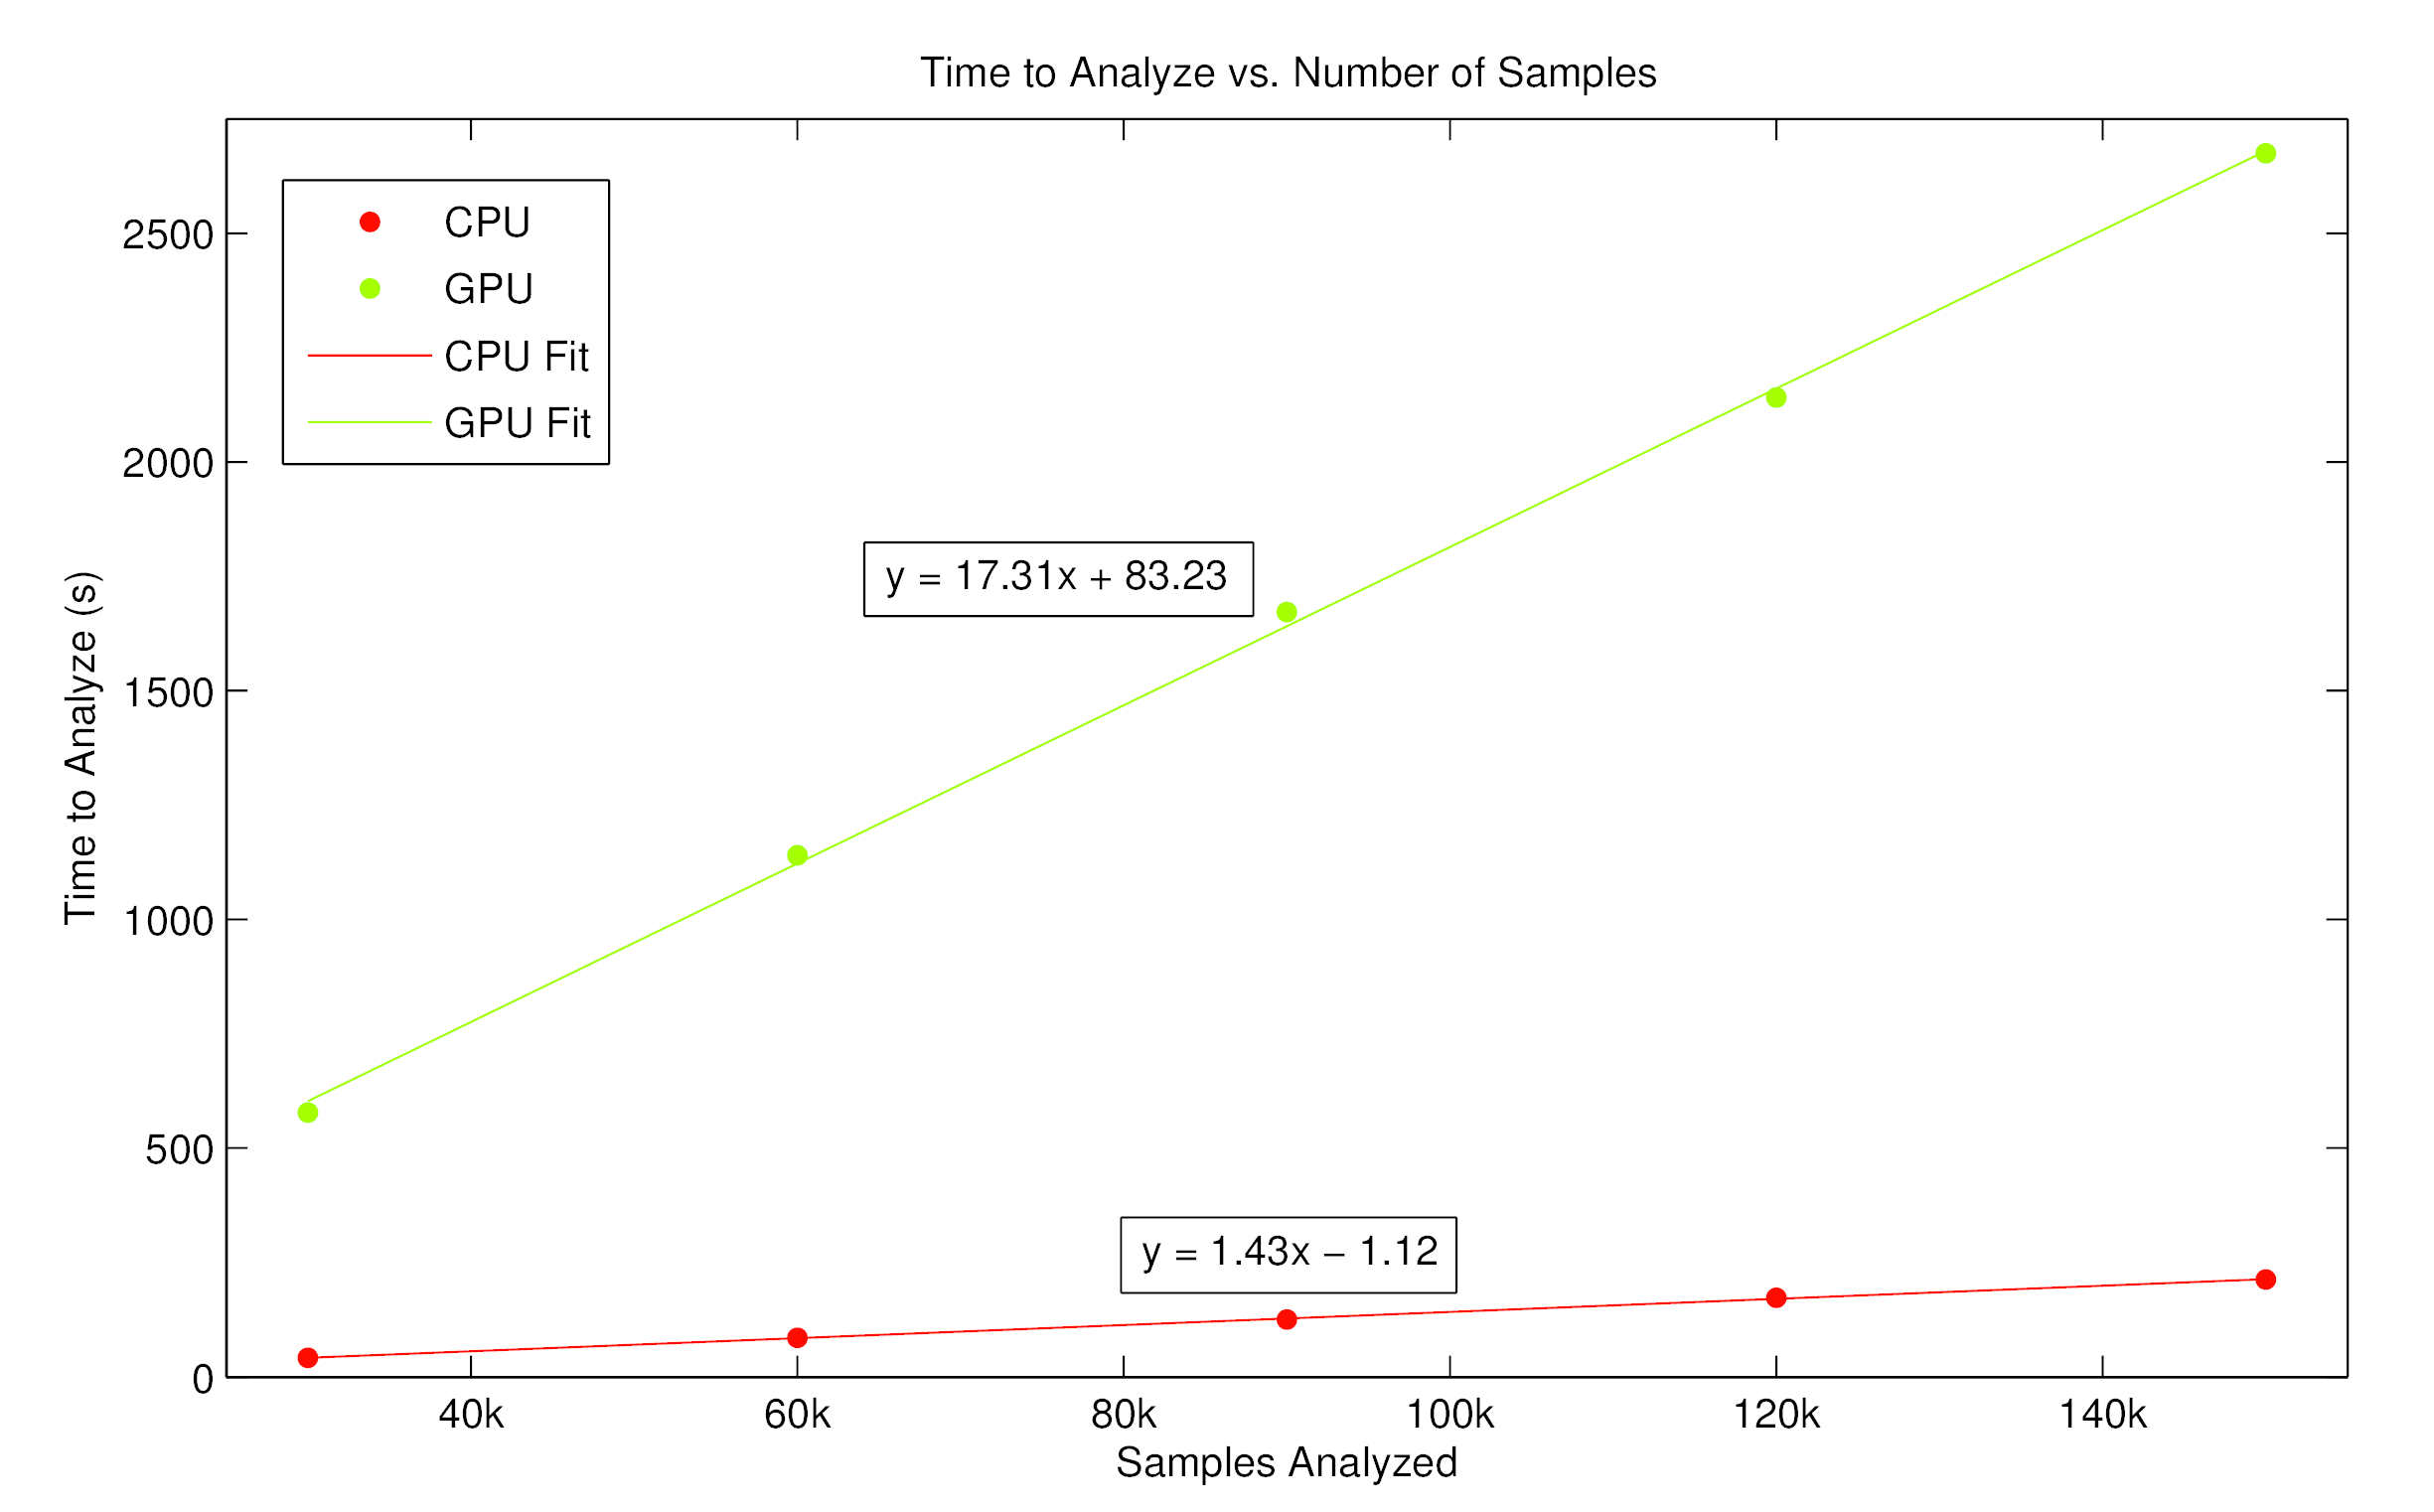
\includegraphics[width=0.75\paperwidth]{Time_vs_Samples.png}
    \caption{Plot of performance based on sample size}
	\label{fig:samples}
\end{figure}

The second experiment tested the performance of LSPI with a constant number of samples while the basis size increased. The experiment was setup by collecting $10,000$ samples from an agent following a random policy with a $25\%$ exploration rate. These samples were then used to train agents with basis functions which ranged in size from $30$ to $258$. As with the samples scaling experiment, every attempt was made to ensure these experiments were completed in identical environments. Due to the variance we witnessed in our experiments we repeated this training for each agent three times for both the CPU and GPU implementation. The results are graphed with fit lines in Figure \ref{fig:basis}.

\begin{figure}
    \centering
    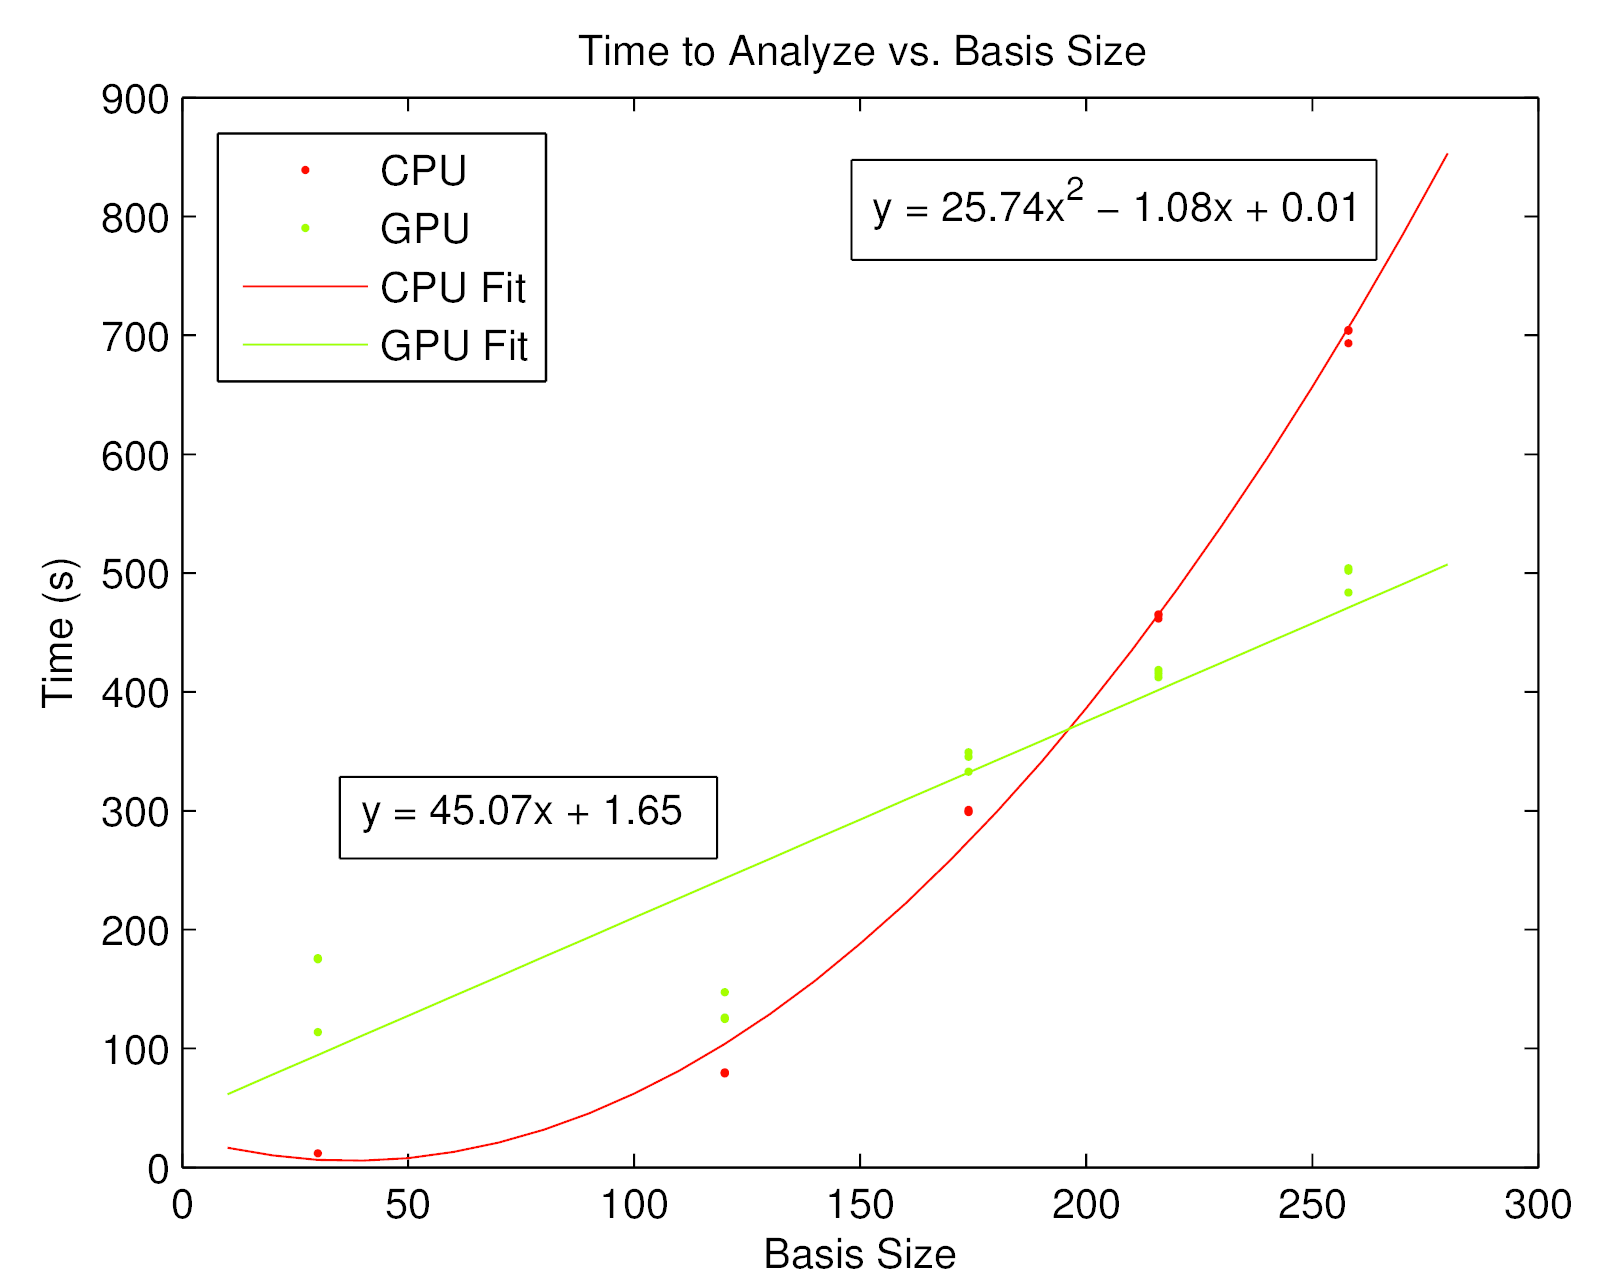
\includegraphics[height=0.33\paperheight]{Time_vs_Basis.png}
    \caption{Plot of performance based on basis size}
    \label{fig:basis}
\end{figure}

Based on the data we collected, it is clear that while the GPU performs slower than the CPU with small basis sizes, the GPU scales well with increasing basis size. For our particular configuration the performance crossover occurs around $200$; however, that intersection point will vary based on the specific hardware configurations as well as the optimizations used to improve performance.

While the speeds we measured on the CPU were relatively stable, we noticed a high level of variance in our measurements for the GPU. Based on our knowledge of how linear algebra operations scale on the GPU, we would expect LSPI to scale approximately linearly on the GPU. Most of our data supports this; however, there are some outliers present on the graph.

When we measured the time to analyze the samples using a basis size of $120$ we were consistently seeing results that were comparable to the amount of time needed to analyze the samples using a basis of size $30$. To understand this result, we must first understand what factors will impact the amount of time needed to execute LSPI.

At its core, LSPI can be viewed as an optimization algorithm which iteratively executes the algorithm LSTD$Q$ in an attempt to locate the policy which maximizes the utility of the agent for the given samples. Depending on both the samples and the basis function used to evaluate the samples, the number of iterations of LSTD$Q$ necessary can change. Looking at Figure \ref{fig:basis} the data shows that although it is less noticeable, all three tests for the CPU also appear under the curve. This suggests that the particular features we selected may have had an impact on the number of iterations of LSTD$Q$ required to converge.

Another potential contributing factor to this result is the nature of the GPU architecture. When code is executed on the GPU, some number of processing units is allocated. The number of processing units allocated does not necessarily correspond with the size of the data input. As a result, there may be processing units which are effectively idle. The end result is that two operations with different input sizes may take the same amount of time. Between the architecture of the GPU and the interaction of the basis features with the speed of convergence, we feel that these results still fall within the expected range.

When it came time to plot fit lines for the data, the choice was obvious for the CPU: the results very clearly represent a second degree polynomial, with $R^2 = 0.99$. For the GPU the choice was less obvious, particularly since the outlier at $120$ made any fit difficult. We chose a linear fit because the data fits a linear model better with the outliers removed. The fit was less consistent for the GPU data with $R^2 = 0.7987$.

It is important to keep in mind that the point at which the GPU overtakes the CPU in performance will vary based on specific hardware configurations, as well as the level of optimization put into the implementation. As stated earlier, we chose to optimize very little to focus on the scaling performance gains. Furthermore, unless the CPU implementation was capable of being optimized at a rate much higher than the GPU optimizations, these performance tweaks would only serve to lower the barrier for seeing improvements with the GPU.

In our experiments we were able to generate very good policies with a very small basis function; however, this is largely due to the amount of hand written scripts our bot relies on to interact with the environment. While this allowed us to test the performance of LSPI under different conditions very well, our AI implementation does not do allow more complex behavior to be learned, limiting the benefits observed using reinforcement learning.

To intuitively understand the benefits of a large basis function, consider designing an AI agent for Quake III from the ground up. In order to manage the complexity of the environment, it is helpful to have some basic actions available to the agent: \emph{attack}, \emph{get health}, \emph{get weapon}, \emph{get armor}, \emph{get powerup}, \emph{search for enemy}, \emph{defend location}, \emph{flee from enemy}, \emph{change weapon}, \emph{reload}. Already our agent has more actions available than the implementation was used for testing.

Now consider what information would be useful in order to make intelligent decisions. First and foremost, the agent needs information on its own state: \emph{health}, \emph{armor}, \emph{equipped weapon}, \emph{available weapons}, \emph{equipped ammo}, \emph{available ammo}. Keep in mind that some of these features, such as equipped weapon and available weapons, would need to be represented by multiple values in the basis. In fact, representing this information in Quake III would already result in a basis with $23$ values which must be repeated for each of the $10$ actions we have defined for a total size of $230$, and we still lack the information to make more complex decisions such as how to choose an area to defend.

\subsection{Impact of Increasing Basis Size}

To empirically demonstrate the impact of increasing the basis size we used an LSPI agent to solve the \emph{inverted pendulum} problem. The problem requires an agent to balance an inverted pendulum attached to a cart by applying one of three actions: left force (-75 Newtons), right force (75 Newtons), or no force (0 Newtons). All actions have noise added uniformly from $-10$ to $10$. The state space is continuous and composed of the vertical angle $\theta$ and the angular velocity $\dot{\theta}$ of the pendulum. The transitions are governed by the following equation \cite{lspi}:

\begin{equation}
    \ddot{\theta} = \frac{g sin(\theta) 0 \alpha ml(\dot{\theta})^2 sin(2\theta)/2 - \alpha cos(\theta)u}{4l/3 - \alpha ml cos^2(\theta)}
\label{eq:pendulum}
\end{equation}
where $g$ represents the gravity constant, $m$ is the pendulum mass, $M$ is the cart mass, $l$ is the pendulum length, $\alpha = 1/(m + M)$, and $u$ is the noisy input. The simulation steps every 0.1 seconds, selecting the agent's action at the beginning of the step and keeping it constant until the next action is selected. If $|\theta| \geq \pi/2$ the pendulum is considered horizontal and receives a reward of $-1$, otherwise the agent receives a reward of 0.

For our test we used the following values:
\[
    \begin{aligned}
        g &= 29.4 m/s^2 \\
        m &= 2.0 kg \\
        M &= 8.0 kg \\
        l &= 3.0 m
    \end{aligned}
\]
and a discount factor of 0.95. The basis function was created by generating $N$ Gaussian functions arranged over the 2-dimensional state space and including a constant factor of $1$. For state $s = (\theta,\dot{\theta})$ and some action $a$, all values are $0$ except for the active block for $a$ which is represented by:
\[
    \big(1, e^{-\frac{||s - \mu_1||^2}{2\sigma^2}}, e^{-\frac{||s - \mu_2||^2}{2\sigma^2}}, \dots, e^{-\frac{||s - \mu_N||^2}{2\sigma^2}}\big)^T
\]
where $\mu_i$ represents a point in the space $\theta \times \dot{\theta}$ and $\sigma^2 = 1$. Specifically, the values for $\mu$ were selected by choosing $N$ uniformly spaced discrete pairs $(\theta, \dot{\theta})$ such that $\theta \in [-\pi/2, \pi/2]$ and $\dot{\theta} \in [-1, 1]$. 

Training samples were collected from random episodes: the pendulum started at a position near $(0,0)$ and the agent selected actions at random. The average length of each episode was 16, generating about 16 samples. Figure \ref{fig:pendulum} shows the performance of policies created for varying number of training episodes.

\begin{figure}
	\centering
		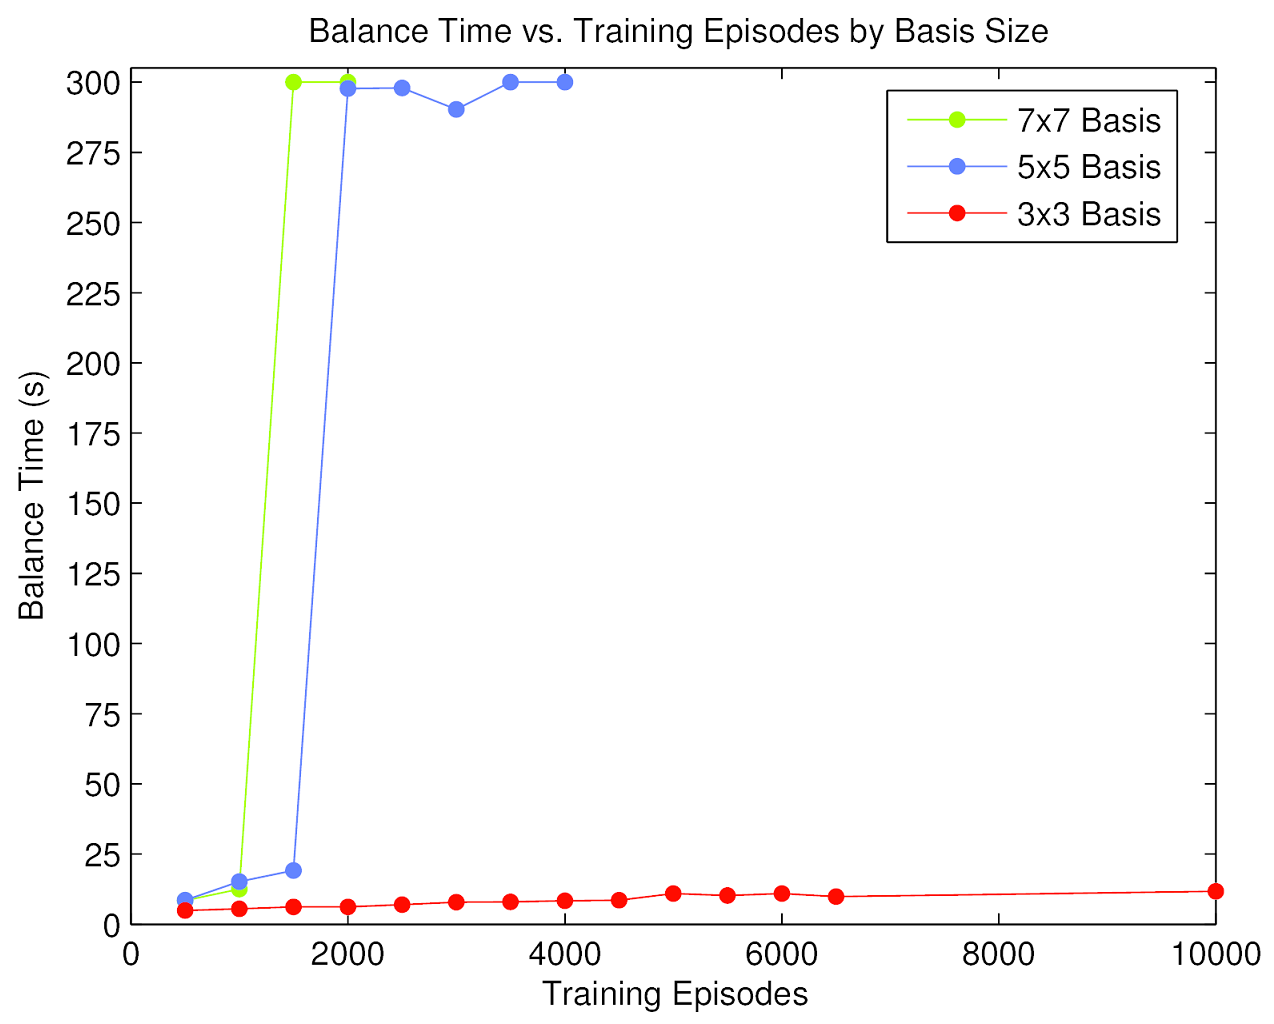
\includegraphics[width=0.33\paperheight]{Balance_vs_Samples.png}
	\label{fig:pendulum}
    \caption{LSPI Inverted Pendulum: Average balancing time}
\end{figure}

If the agent balances for $300$ seconds the episode comes to an end as it is likely the agent has developed an optimal policy. For each basis size we increased the number of training episodes by $500$ until two perfect results were achieved. The smallest basis was tested up $6.5$k training samples before we skipped to $10$k and then $15$k (not shown). None of these tests showed any significant improvement so we discontinued testing.

The numbers in the legend of Figure \ref{fig:pendulum} lists the basis size in terms of the number of discrete values for $\theta$ and $\dot{\theta}$ selected from. For example the smallest basis size was created by selecting points from $\{-\pi/2, 0, \pi/2\} \times \{-1, 0, 1\}$.

The experiment results demonstrate that the size of the basis function can have an impact on two important convergence factors. First, the smallest basis function did not contain enough information to converge on an optimal solution, suggesting that a larger basis function may be required in order to implement an effective agent. Second, the largest basis function needed fewer samples to converge when compared to the medium basis function. In some environment this may provide a performance benefit while in others it is desirable because the agent can learn effective policies with less training time.

\section{Online LSPI}

The algorithm for Online LSPI is described in \ref{chap:implementation}. To evaluate its effectiveness as an alternative to traditional online algorithms we implemented OLPOMDP and Online LSPI in the Quake III environment and compared their performance and effectiveness.

\subsection{Policy Gradient}

The term \emph{Policy Gradient} describes a class of machine learning techniques which apply gradient ascent optimization to determine the optimal policy. Given the policy value function, $p(\theta)$, policy gradient algorithms can be succinctly described by the following formula:

\[
    \theta_{n+1} = \theta_{n} + \alpha\nabla_\theta p(\theta_{n})
\]
where $\theta$ represents the policy parameters and $\alpha$ is referred to as the step size or learning rate \cite{norvig}\cite{bishop}.

Before we estimate $\nabla_\theta p(\theta)$, we must ensure that $p(\theta)$ is differentiable with respect to $\theta$. Assume we have a basis function, $J_\theta(s,a)$ which is used to generate a policy as follows:

\[
    \pi_\theta(s,a) = \argmax_a J_\theta(s,a)
\]
The use of the $argmax$ function may result in a discontinuous distribution. This can be fixed by using a probabilistic policy \cite{olpomdp:lecture}:

\begin{equation}
\label{eq:grad:policy}
    \pi_\theta(s,a) = Pr(a|s) = \frac{e^{J_\theta(s,a)/T}}{\sum\limits_{a'\in A} e^{J_\theta(s,a')/T}}
\end{equation}

To estimate the gradient from samples we use the following formula:
\begin{equation}
\label{eq:grad}
    \begin{aligned}
        \nabla_\theta p(\theta) &= \sum_a\pi_\theta(s_0,a)g_\theta(s_0,a)R(a) \\
        g_\theta(s_0,a) &= f_\theta(s_0, a) - \sum\limits_{a'} \pi_\theta(s_0,a')f_\theta(s_0,a')
    \end{aligned}
\end{equation}

Equation \ref{eq:grad} is the basis for an online algorithm called OLPOMDP \cite{olpomdp}. Intuitively, the algorithm estimates the gradient using Monte Carlo techniques: execute the policy while making small changes to $\theta$. Because we use Equation \ref{eq:grad:policy} to select actions, our agent will naturally explore the environment. With each action we then update the value $e$, called the eligibility trace, by estimating the value of the gradient for that action.

The pseudocode for OLPOMDP is given in Algorithm \ref{olpomdp}. Notice that instead of updating $\theta$ directly the value $e$, called the eligibility trace, is used as an intermediary. The eligibility trace represents the discounted sum of gradients over previous state-action pairs and is used to update $\theta$ according to the reward given for the corresponding action. The value $\beta$ is referred to as the bias and controls the weight of previous experiences in the environment. Increasing $\beta$ biases the algorithm toward past experiences while also increasing the variance. 

\begin{algorithm}
\caption{OLPOMDP}
\label{olpomdp}
    {\fontsize{12}{10}\selectfont
    \begin{algorithmic}[1]
        \REQUIRE
            \begin{itemize} 
                \item $\beta \in [0,1)$ 
                \item $T > 0$ 
                \item $\theta_0 \in \mathbb{R}^K$ 
            \end{itemize}
    \STATE Set $e = 0$
    \FOR{$t = 0$ to $\infty$}
        \STATE Observe the current state, $s$
        \STATE Select action $a$ according to $\pi_\theta(s)$
        \STATE Execute $a$
        \STATE Observe reward $r$
        \STATE $e \leftarrow \beta e + f(s,a) - \sum\limits_{a'}\pi_\theta(s,a')f_\theta(s,a')$
        \STATE $\theta \leftarrow + \alpha \cdot r \cdot e$
    \ENDFOR
    \end{algorithmic}
    }
\end{algorithm}

\subsection{Evaluation of Online Algorithms}

For the purpose of comparison both agents were tested using GPU acceleration in identically configured Quake III matches. All bots were given the personality of \emph{Ranger} to ensure no bots, including the Quake III bots, had any unfair advantages in physical characteristics. We evaluated the performance of each agent in a deathmatch against a native bot with no time limit and a 500 kill limit. The difficulty was set to \emph{Bring It On}, the second lowest difficulty level. This provided us the benefit of creating a high contrast between good and bad policies due to the impact on scripted bot behavior. The Online LSPI agent used a discount rate of $0.95$ and an exploration rate of $0.25$. The OLPOMDP agent used $\beta = 0.80$ and a step size of $0.05$.

\begin{figure}
		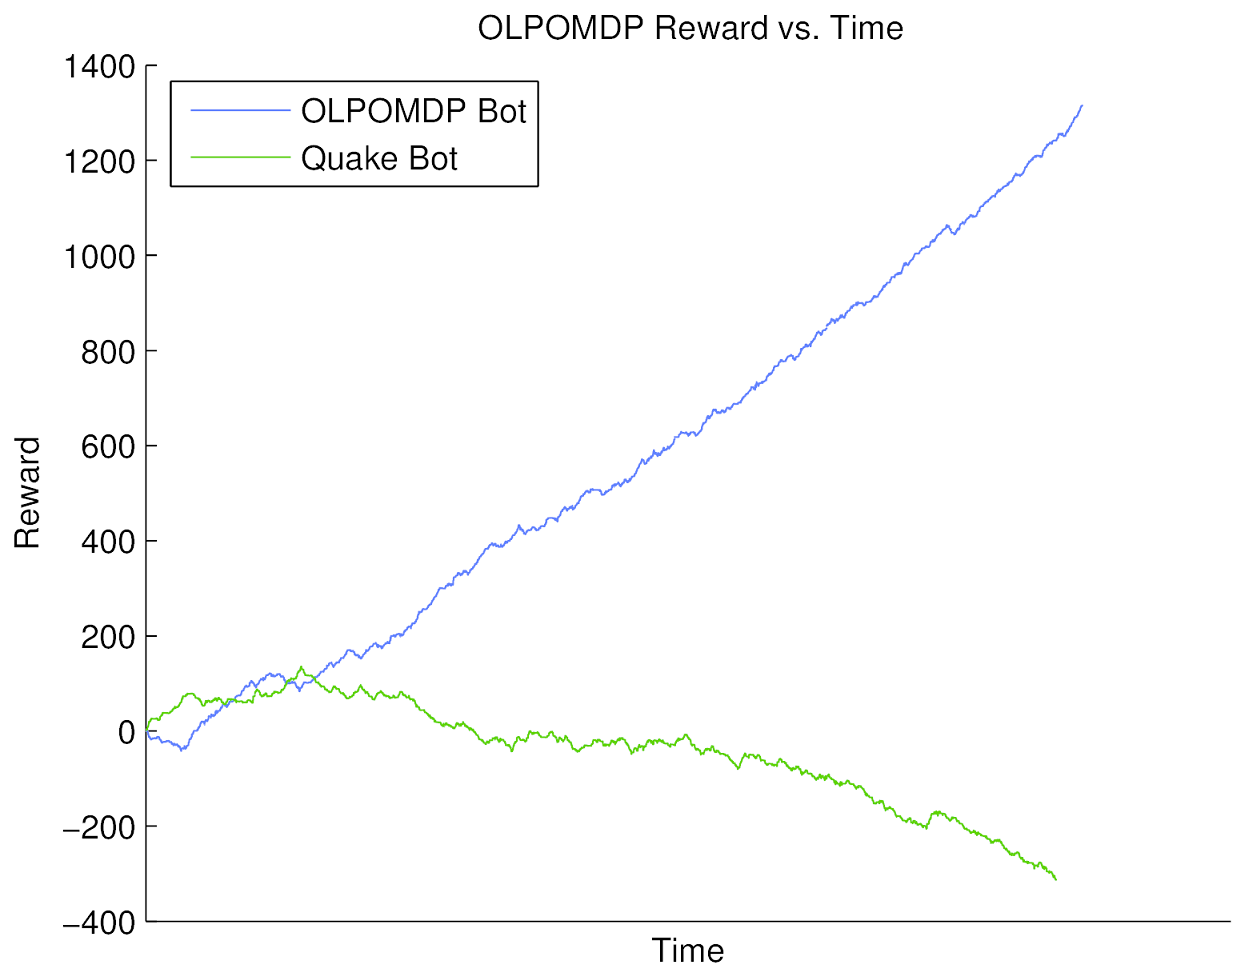
\includegraphics[width=0.5\textwidth]{OLPOMDP_Reward_vs_Time.png}
        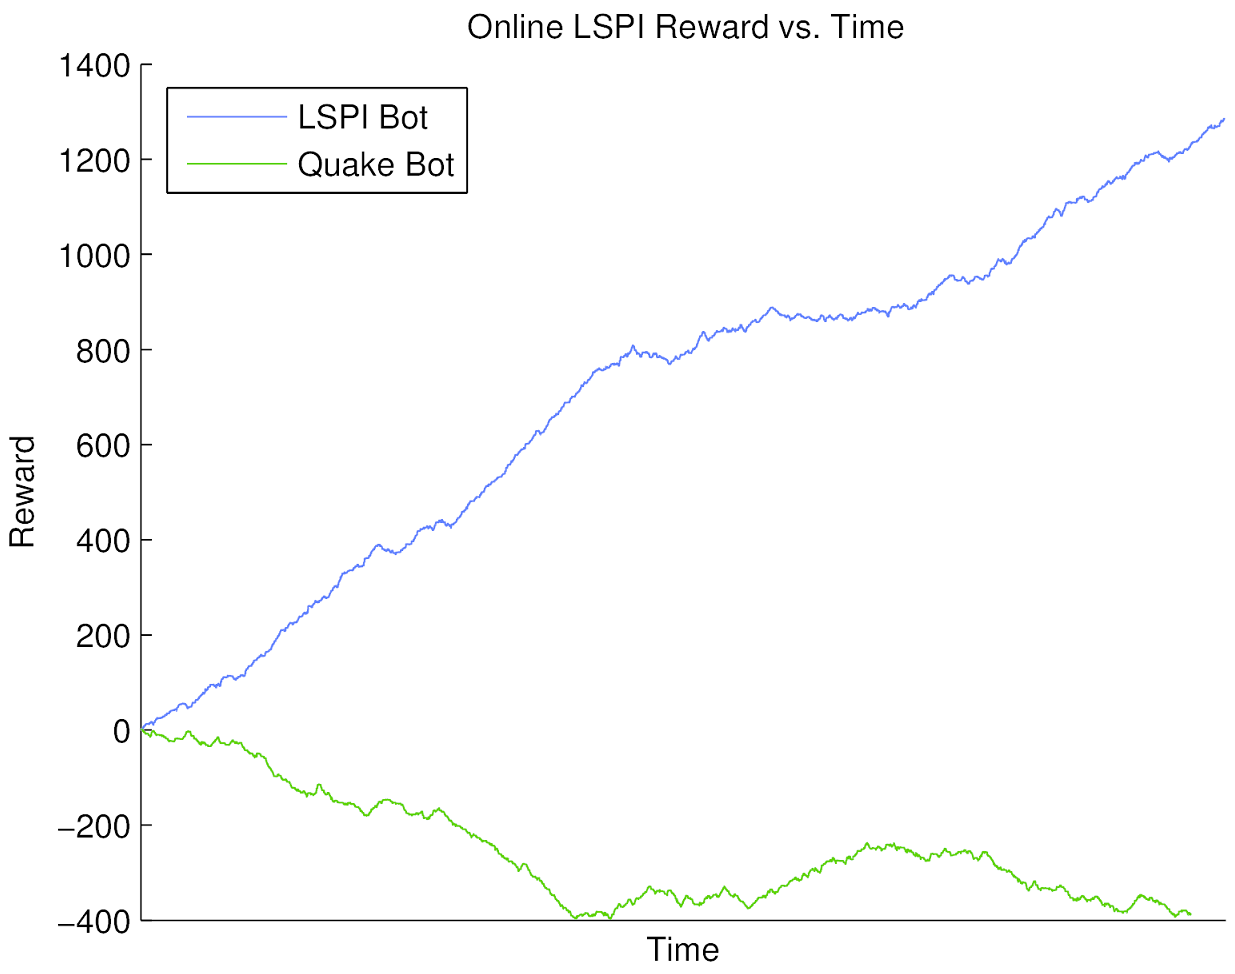
\includegraphics[width=0.5\textwidth]{LSPI_Reward_vs_Time.png}
	\label{fig:online:reward}
    \caption{Online Agent Reward}
\end{figure}

The result of the matches is displayed in Figure \ref{fig:online:reward}. Both the Online LSPI and OLPOMDP agents were able to win when placed against the native bot. In both matches our agents scored approximately twice as many kills as the native bots. While the end result was the same, a few differences are noticeable in the reward graphs. The LSPI agent appeared to start with a better policy, although the OLPOMDP agent was quickly able to overcome this advantage and finish the match with a reward of $1316$ as compared to the LSPI agent with $1286$. In addition, OLPOMDP demonstrated a more stable average reward with the policy changes in LSPI appearing to cause some reward loss. Overall, however, both algorithms performed on par and achieved nearly the same end result.

\begin{figure}
	\centering
		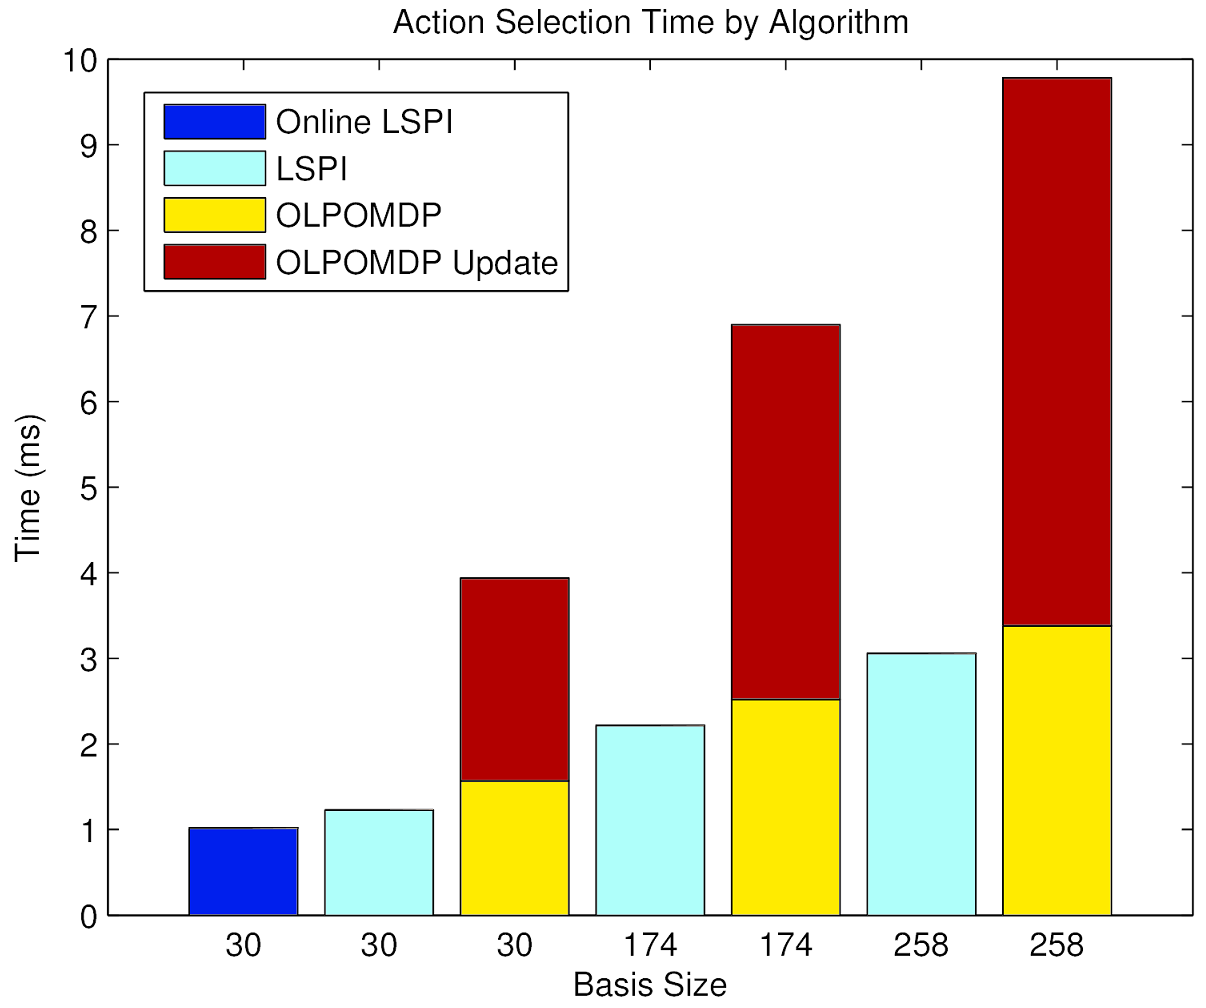
\includegraphics[height=0.33\paperheight]{Action_Selection_Time.png}
	\caption{Average time required to select an action.}
	\label{fig:action:selection}
\end{figure}

Figure \ref{fig:action:selection} shows the average time required to select an action for each agent across the small, medium, and large basis sizes. The values for LSPI and OLPOMDP were selected by tracking the amount of time each action selection operation took over the course of a deathmatch to $50$. The value for Online LSPI was taken from the experiment demonstrated in Figure \ref{fig:online:reward}. For clarity the values for OLPOMDP were split into the update and action selection steps.

We observed that Online LSPI does not appear to suffer any performance loss due to the background updates. To understand this result, recall that GPU operations are generally bound by memory operations. In order to reduce the impact of delays waiting for memory operations to complete the hardware is optimized for fast context switching, allowing multiple programs or operations to interleave rapidly \cite{gpgpu}. 

Because we did not optimize our code to minimize the delay in memory, we do not appear to lose performance when we add simultaneous operations. Note, however, that if we were to optimize all operations it is possible that LSPI would begin to perform better as we approach the GPU's throughput limit. It is also possible that the exploration policy improved performance because the basis function does not need to be computed when a random action is selected.

We observed approximately a factor of 4 speedup when using Online LSPI over OLPOMDP. OLPOMDP appears to be dominated by the update step which consistently takes longer than just selecting an action; however, action selection also takes slightly longer due to the requirement to generate random numbers to follow the probabilistic policy.

\begin{figure}
	\centering
		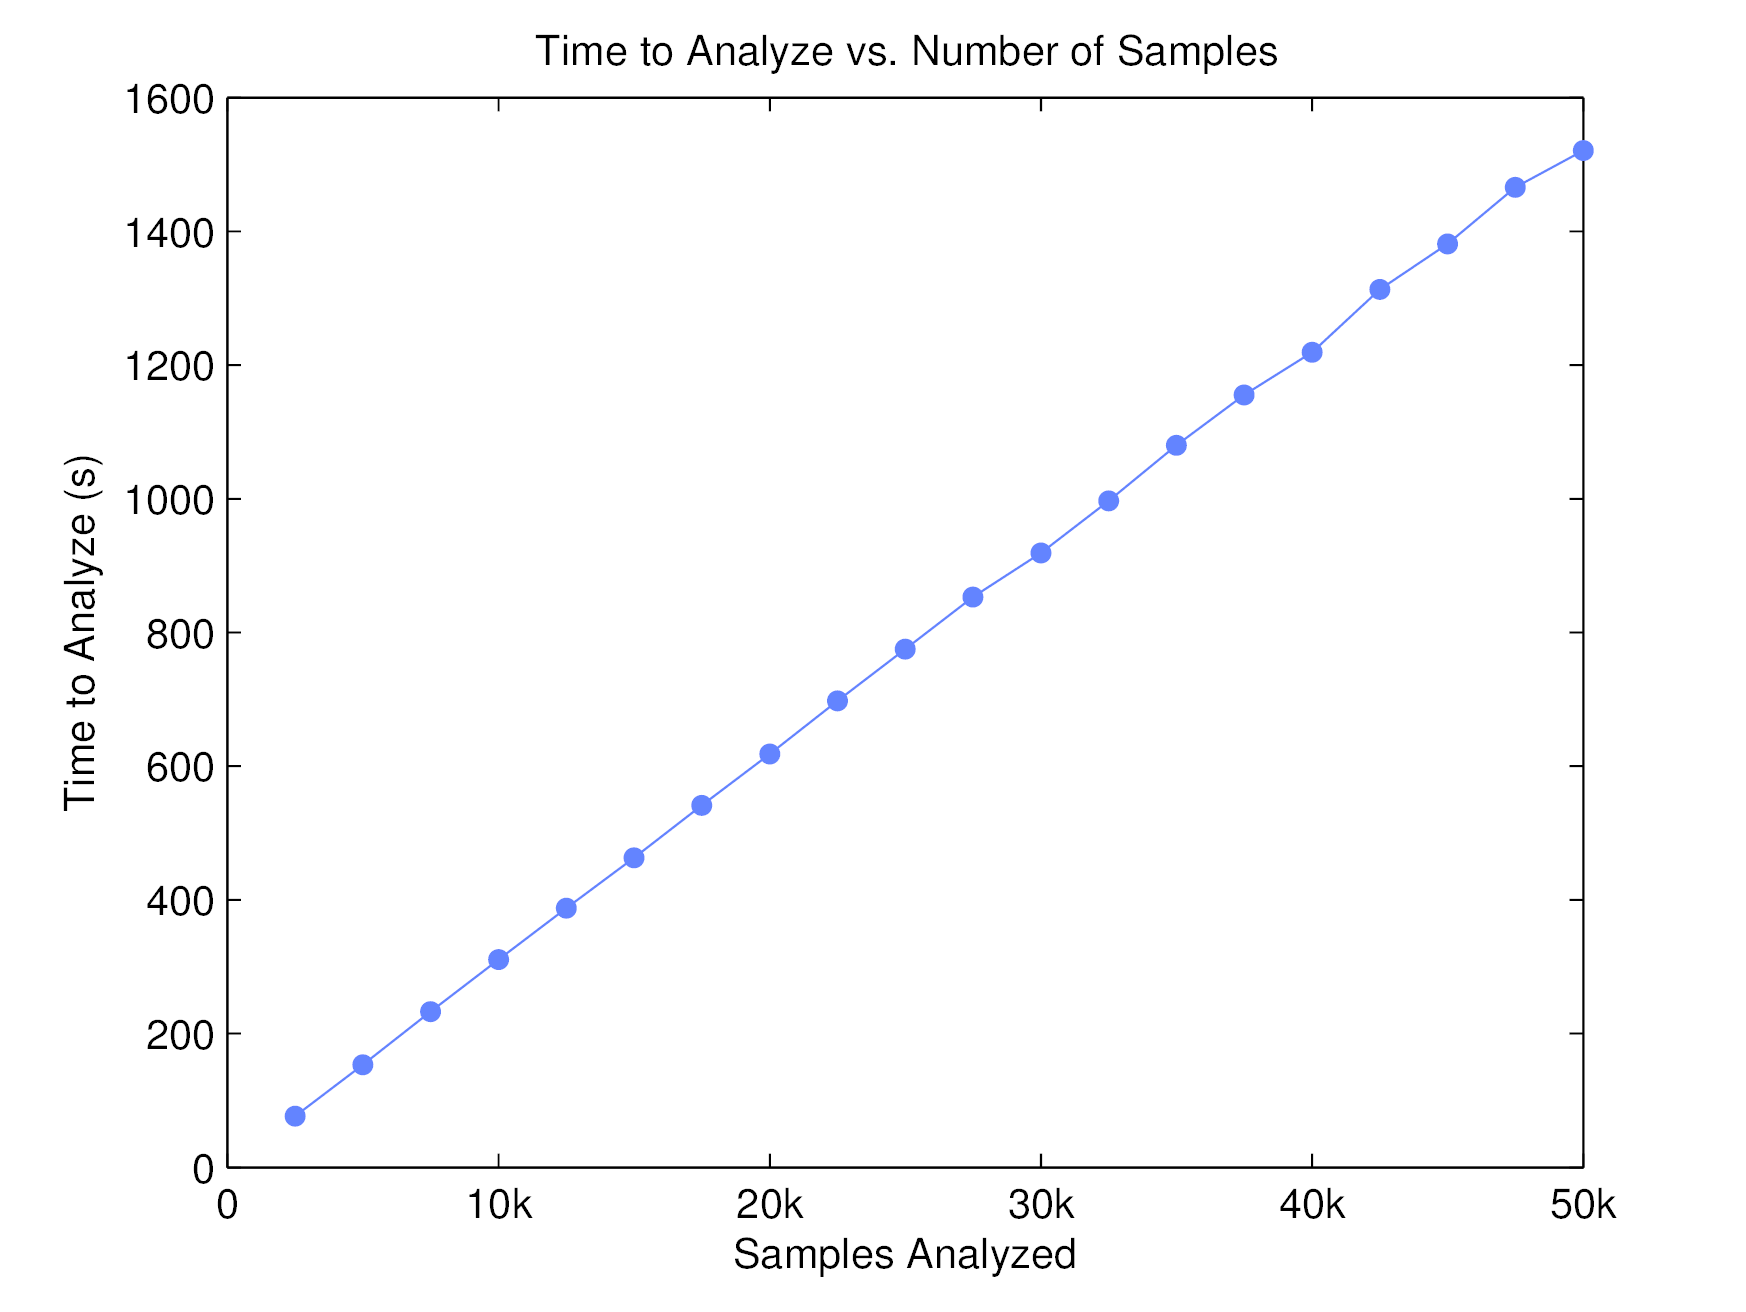
\includegraphics[height=0.33\paperheight]{Online_Time_vs_Samples.png}
	\caption{Time to analyze samples in Online LSPI.}
	\label{fig:online:samples}
\end{figure}

The results in Figure \ref{fig:online:samples} demonstrate the scaling of analysis as samples are collected in Online LSPI. We chose not to directly include the results from \ref{fig:samples}, as they cannot be directly compared. For the tests in samples scaling the samples included the time to load the samples from a file, but in this test the samples were already in memory. Despite this disparity, our test clearly demonstrates no significant performance loss when running online with a speed improvement of $20\%$ over our previous tests and approximately the same scaling factor. Accounting for the file operations it appears that our experiment performed almost identically in online and offline mode. It is worth noting that in a more taxing graphical environment less computing power would be available and we would expect to start seeing performance losses.